\documentclass{article}
\usepackage{graphicx}
%\usepackage{tabular}
\usepackage{hyperref}

\begin{document}
\title{Assignment 2}
\author{Helga Rykov Ibsen}
\date{\today}
\maketitle

\section{Task 2i0}
\begin{enumerate}
  \item
The first method to run an F\# program is to write the code directly in the interactive mode, i.e. the console. The main advantage of using this method is that it produced the result immediately, which might be preferable when writing short programs. Its main disadvantage, though, is its incapability of saving the program. That is, the interactive mode allows to fx get numerous calculations, but it does not save them as a coherent program/file.

\item
The second method to run an F\# program is to use the interpreter mode (fx by using Emacs editor), that allows you both to write the code and save it as a single file. The main advantage of using this mode is that it allows writing longere and more complex programs as well as saving them. Besides, in case the program is to be executed only once, then it's faster to execute an fsx-file with fsharpi than to compile it with fsharpc and execute it with mono.  Its main disadvantage consists in its incapabilily of executing the commands immediately, which is possible with the interactive mode.

\item
The third method to run an F\# program is by using the compiler mode that translates the source code into a format that can be executed by a computer and stores the result in the executable file. Its main advantage relates to running/executing large programs numerous times, because it's much faster to use the compiled version by running mono than to use the interpreter mode, fsharpi. Its main disadvantage is that it takes slightly longer time to execute a code, when we run it once by using the compiler than by using the interactive mode fsharpi. Besides, running the compiler produces additinal files, which might not be appropriate for short programs.

\end{enumerate}
To put it in a nutshell, programs are written in programming languages, such as F\#. But programming languages are abstract and they cannot be read by a computer. That means that for a computer to process an input in F\#, the code written in say F\# needs to be compiled into the assembly language. Eventually, the input in the assemby language needs to be interpreted into the machine code, because computers differ in terms of their processors. That is, we need to use mono in order to compile the assemby language to native code.


\section{Task 2i1}
\textbf{The rule of thumb} is that expressions, such as \"hello world\", written in fsharpi produce output ONLY if they're interpreted with the fsharpc and then executed with mono.
To extract the first and the second word from the string \"hello world\", I started out in the fsharpi mode and tested the printfn-funktion in combination with the desired output. Then I ran fsharpc and mono in the console and got the result. In case at hand (see Figure \ref{output1}), I
\begin{enumerate}
\item asked the computer to print the string \"hello world\";
\item asked the computer to extract the word \"world'' by specifying the desired index-frame [6..];
\item asked the computer to extract the word \"hello'' by specifying the desired index-frame [0..4].
\end{enumerate}

\begin{figure}[h!]
  \centering
 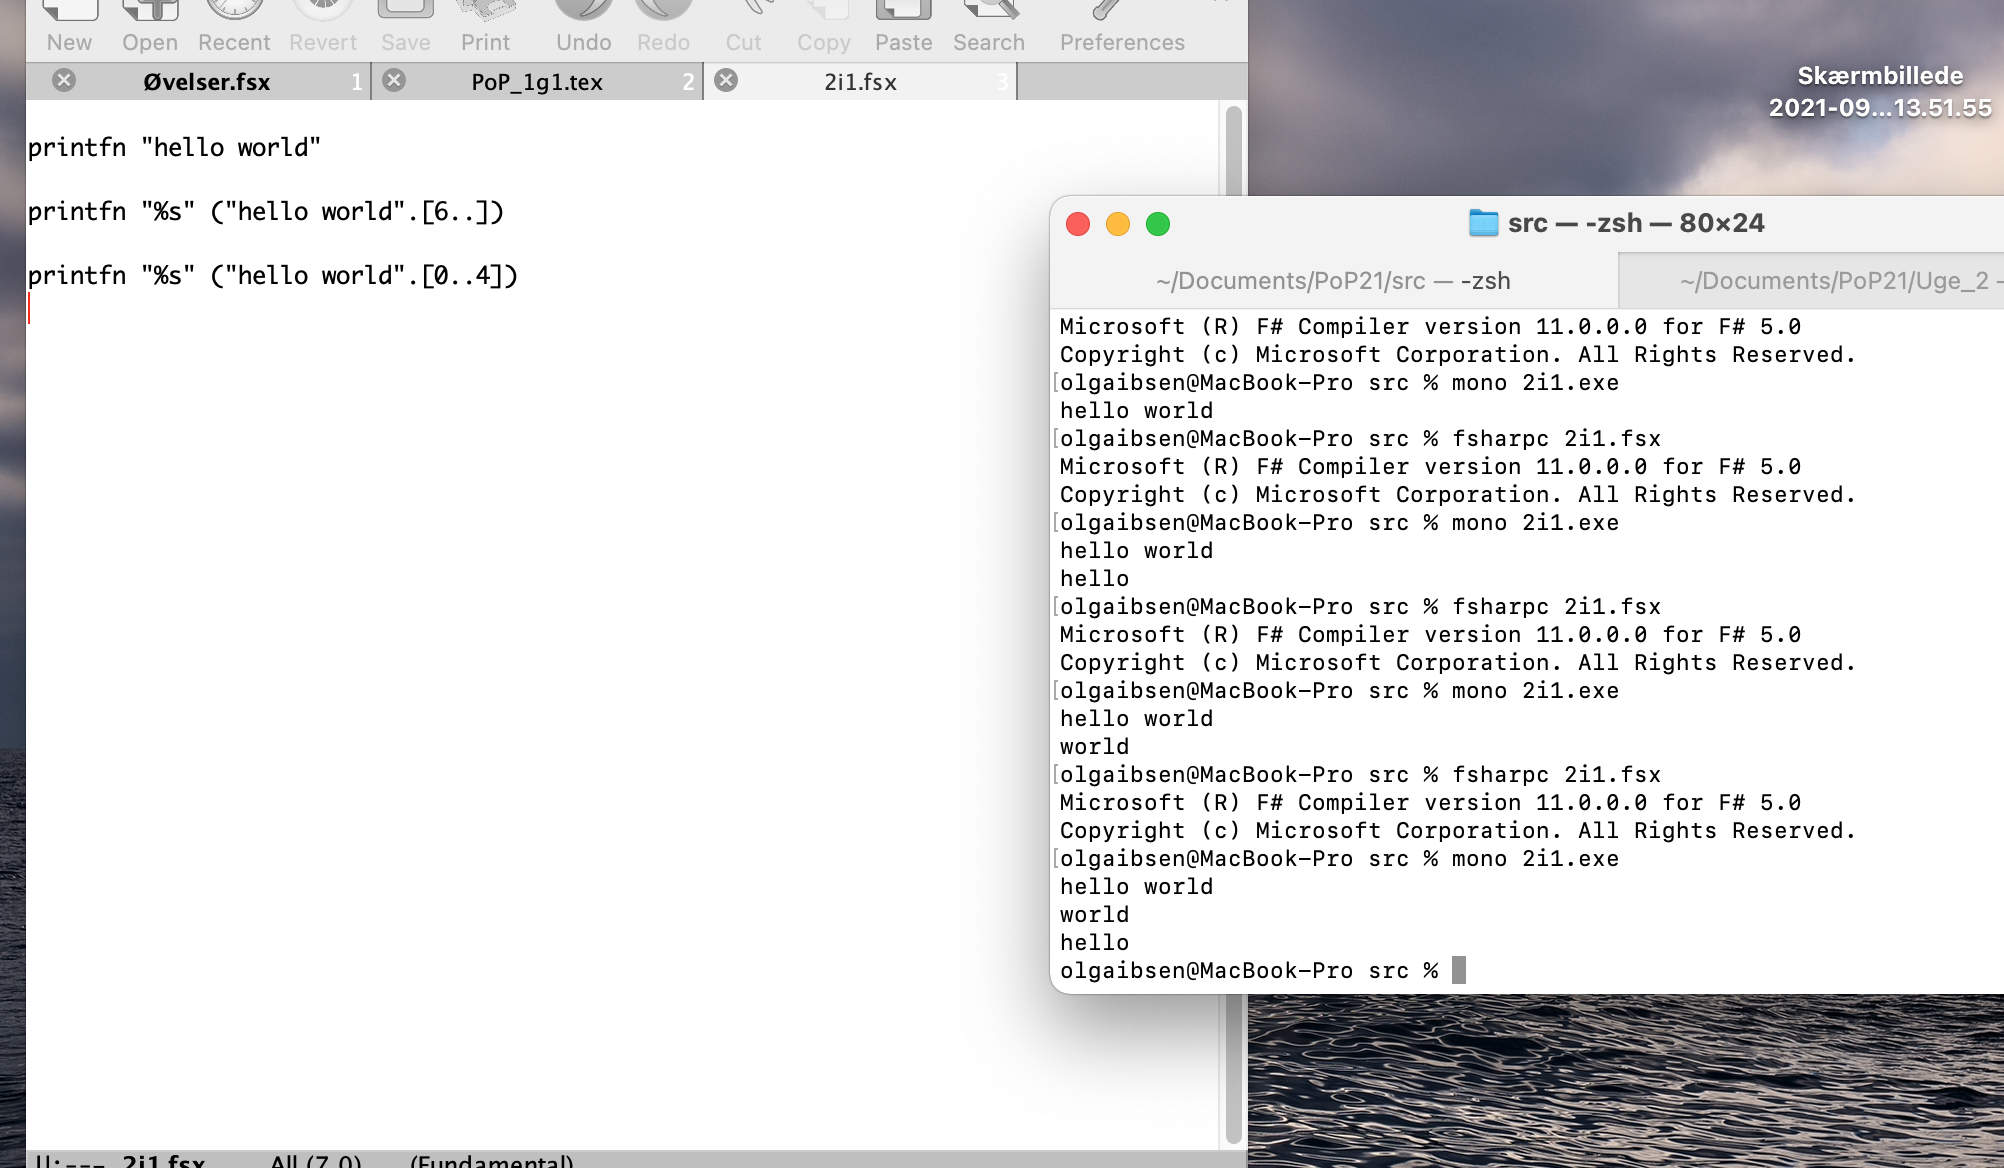
\includegraphics [width=10cm]{Figure_1.png}
 \caption{Slicing operation: Hello world}
 \label{output1}
\end{figure}
To sum up, I succeeded in achieving the desired output by following the procedure described above in 1.-3.

\section{Task 2i2}
The final results for converted numbers are presented in the Table \ref{output2} below:
f\begin{table}[h!]
\begin{center}
\begin{tabular}{|c|c|c|c|}
 \hline
Decimal & Binary &Hexadecimal & Octal  \\
 \hline
 10  & 1010  & a & 12  \\
  \hline
  21 & 10101 & 15 & 25  \\
 \hline
47  &101111  &2f & 57  \\
 \hline
59 & 111011  &3b & 73  \\
  \hline
\end{tabular}
\end{center}
 \caption{The overall results for converted numbers}
 \label{output2}
\end{table}
\newline
Consider Figure \ref{output3} for a pen-and-paper calculation of the conversion procedure from a decimal number 10 to a binary number.
\begin{figure}[h!]
  \centering
 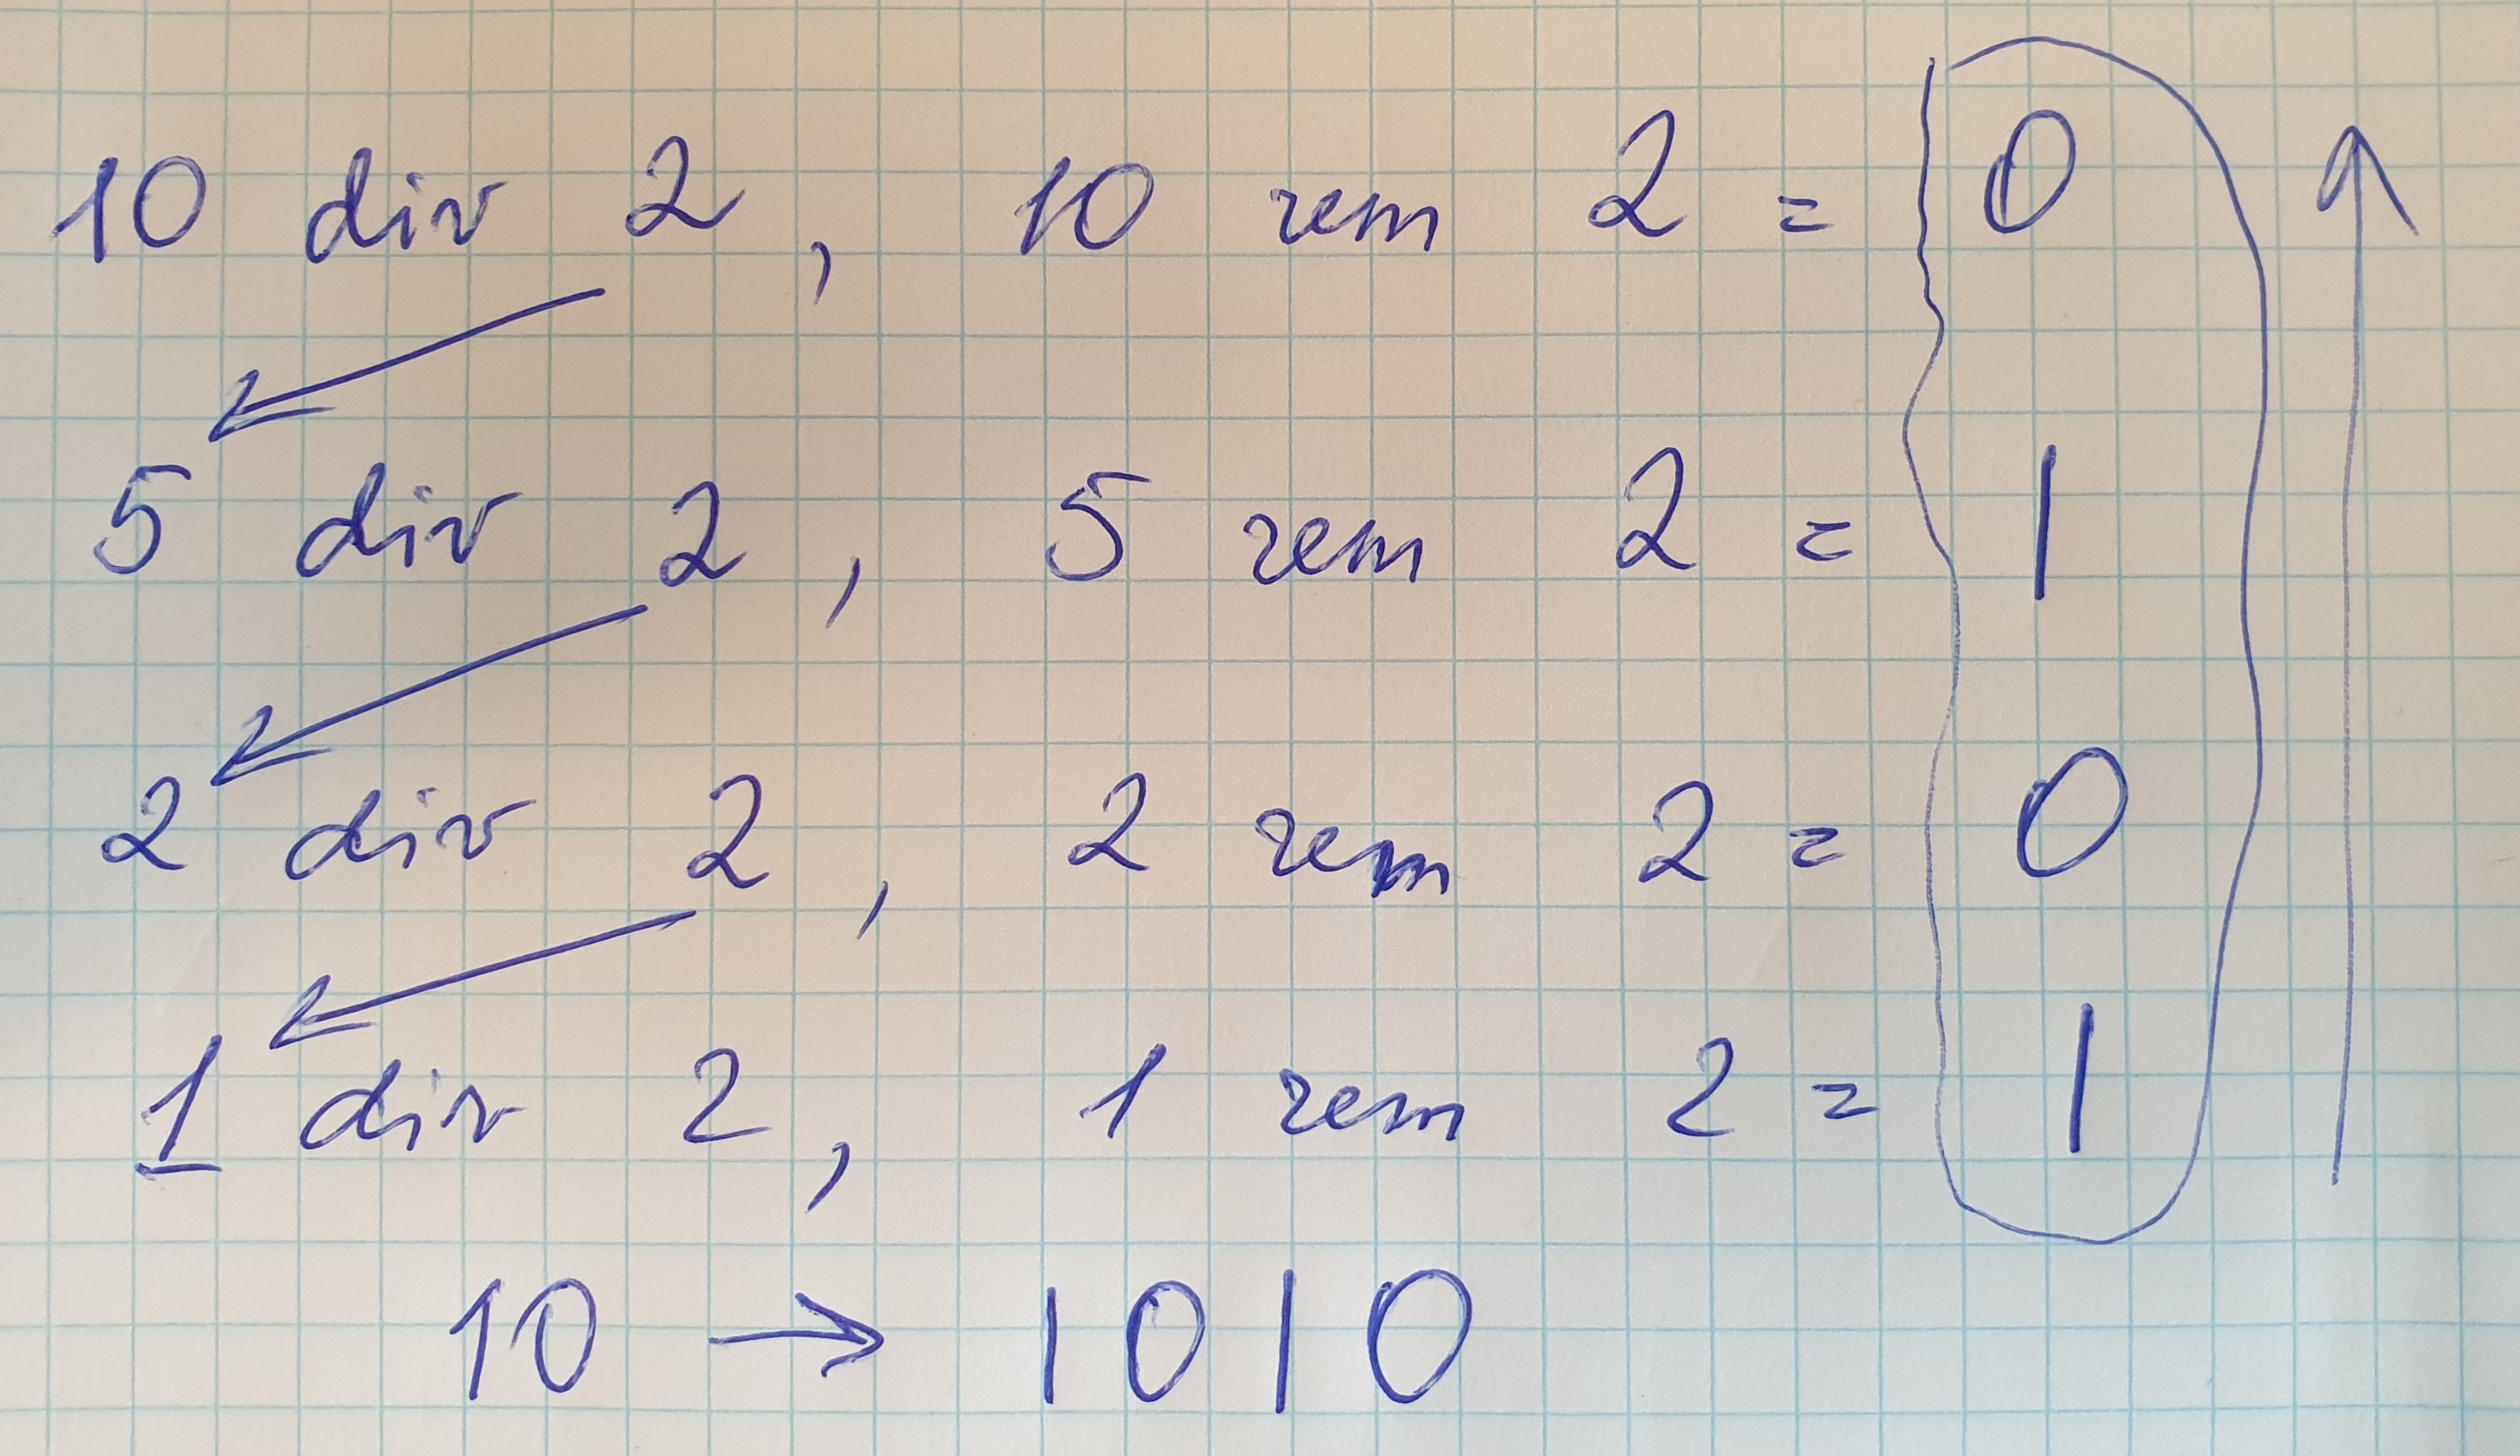
\includegraphics [width=10cm]{Decimal_to_binary.jpg}
 \caption{Decimal to binary}
 \label{output3}
\end{figure}
\newline
Consider Figure \ref{output4} for a pen-and-paper calculation of the conversion procedure from a binary to a decimal number.
\begin{figure}[h!]
  \centering
 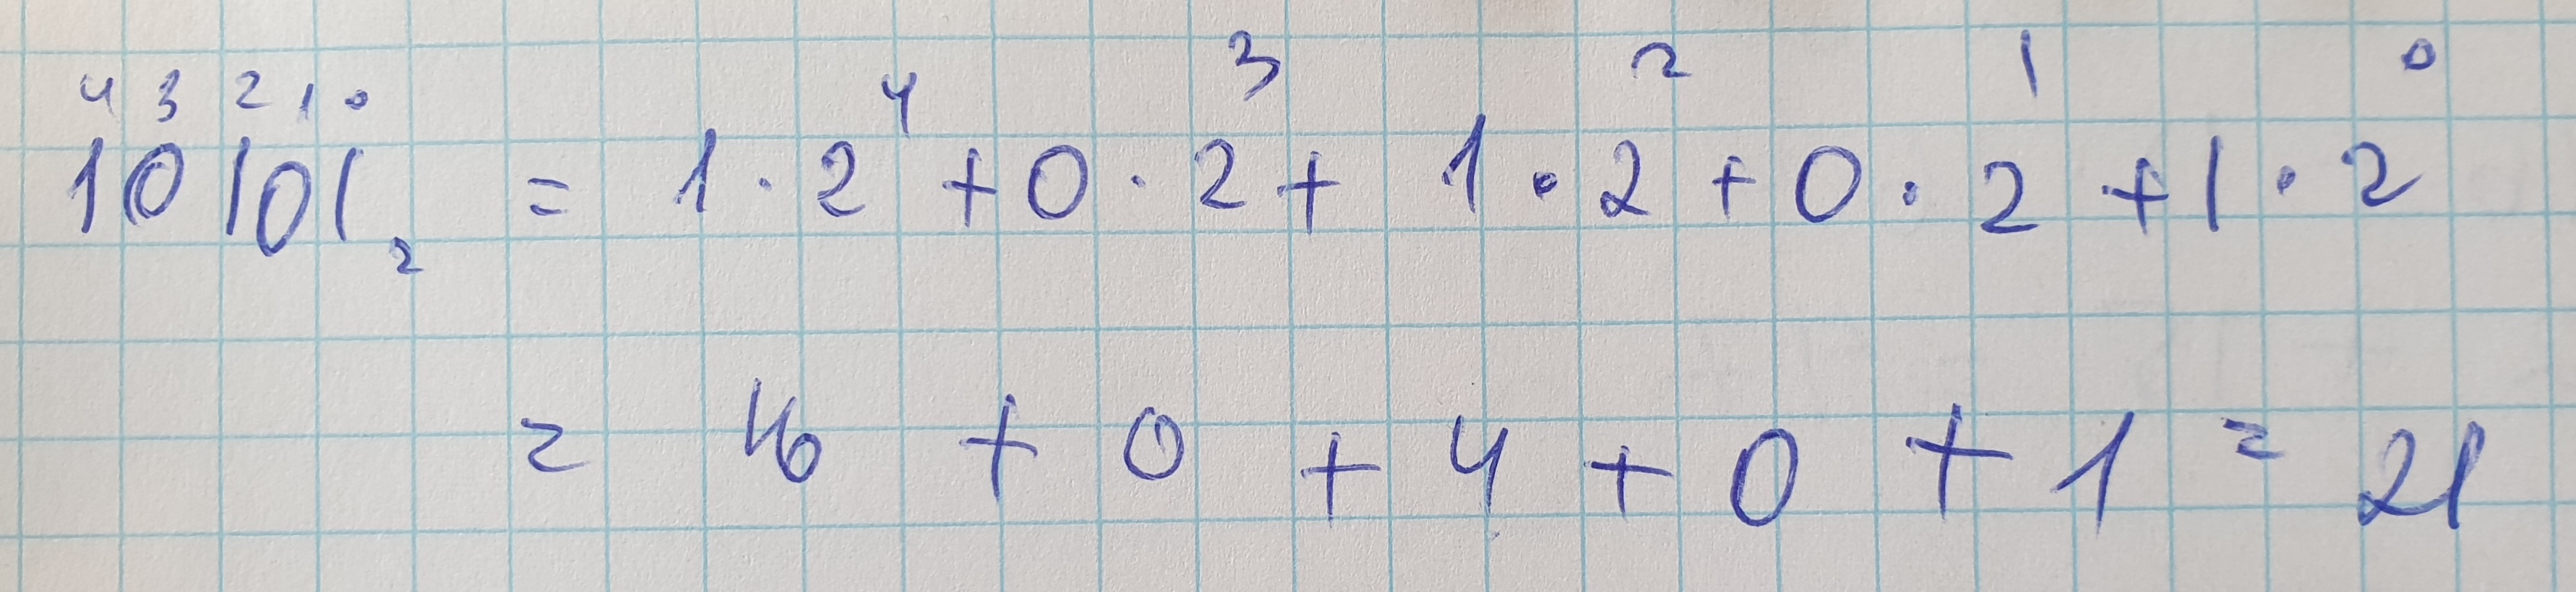
\includegraphics[scale=0.1]{Binary_to_decimal.jpg}
 \caption{Binary to decimal}
 \label{output4}
\end{figure}
\newline
Consider Figure \ref{output5} for a pen-and-paper calculation of the conversion procedure from a binary to a hexadecimal.
\begin{figure}[h!]
  \centering
 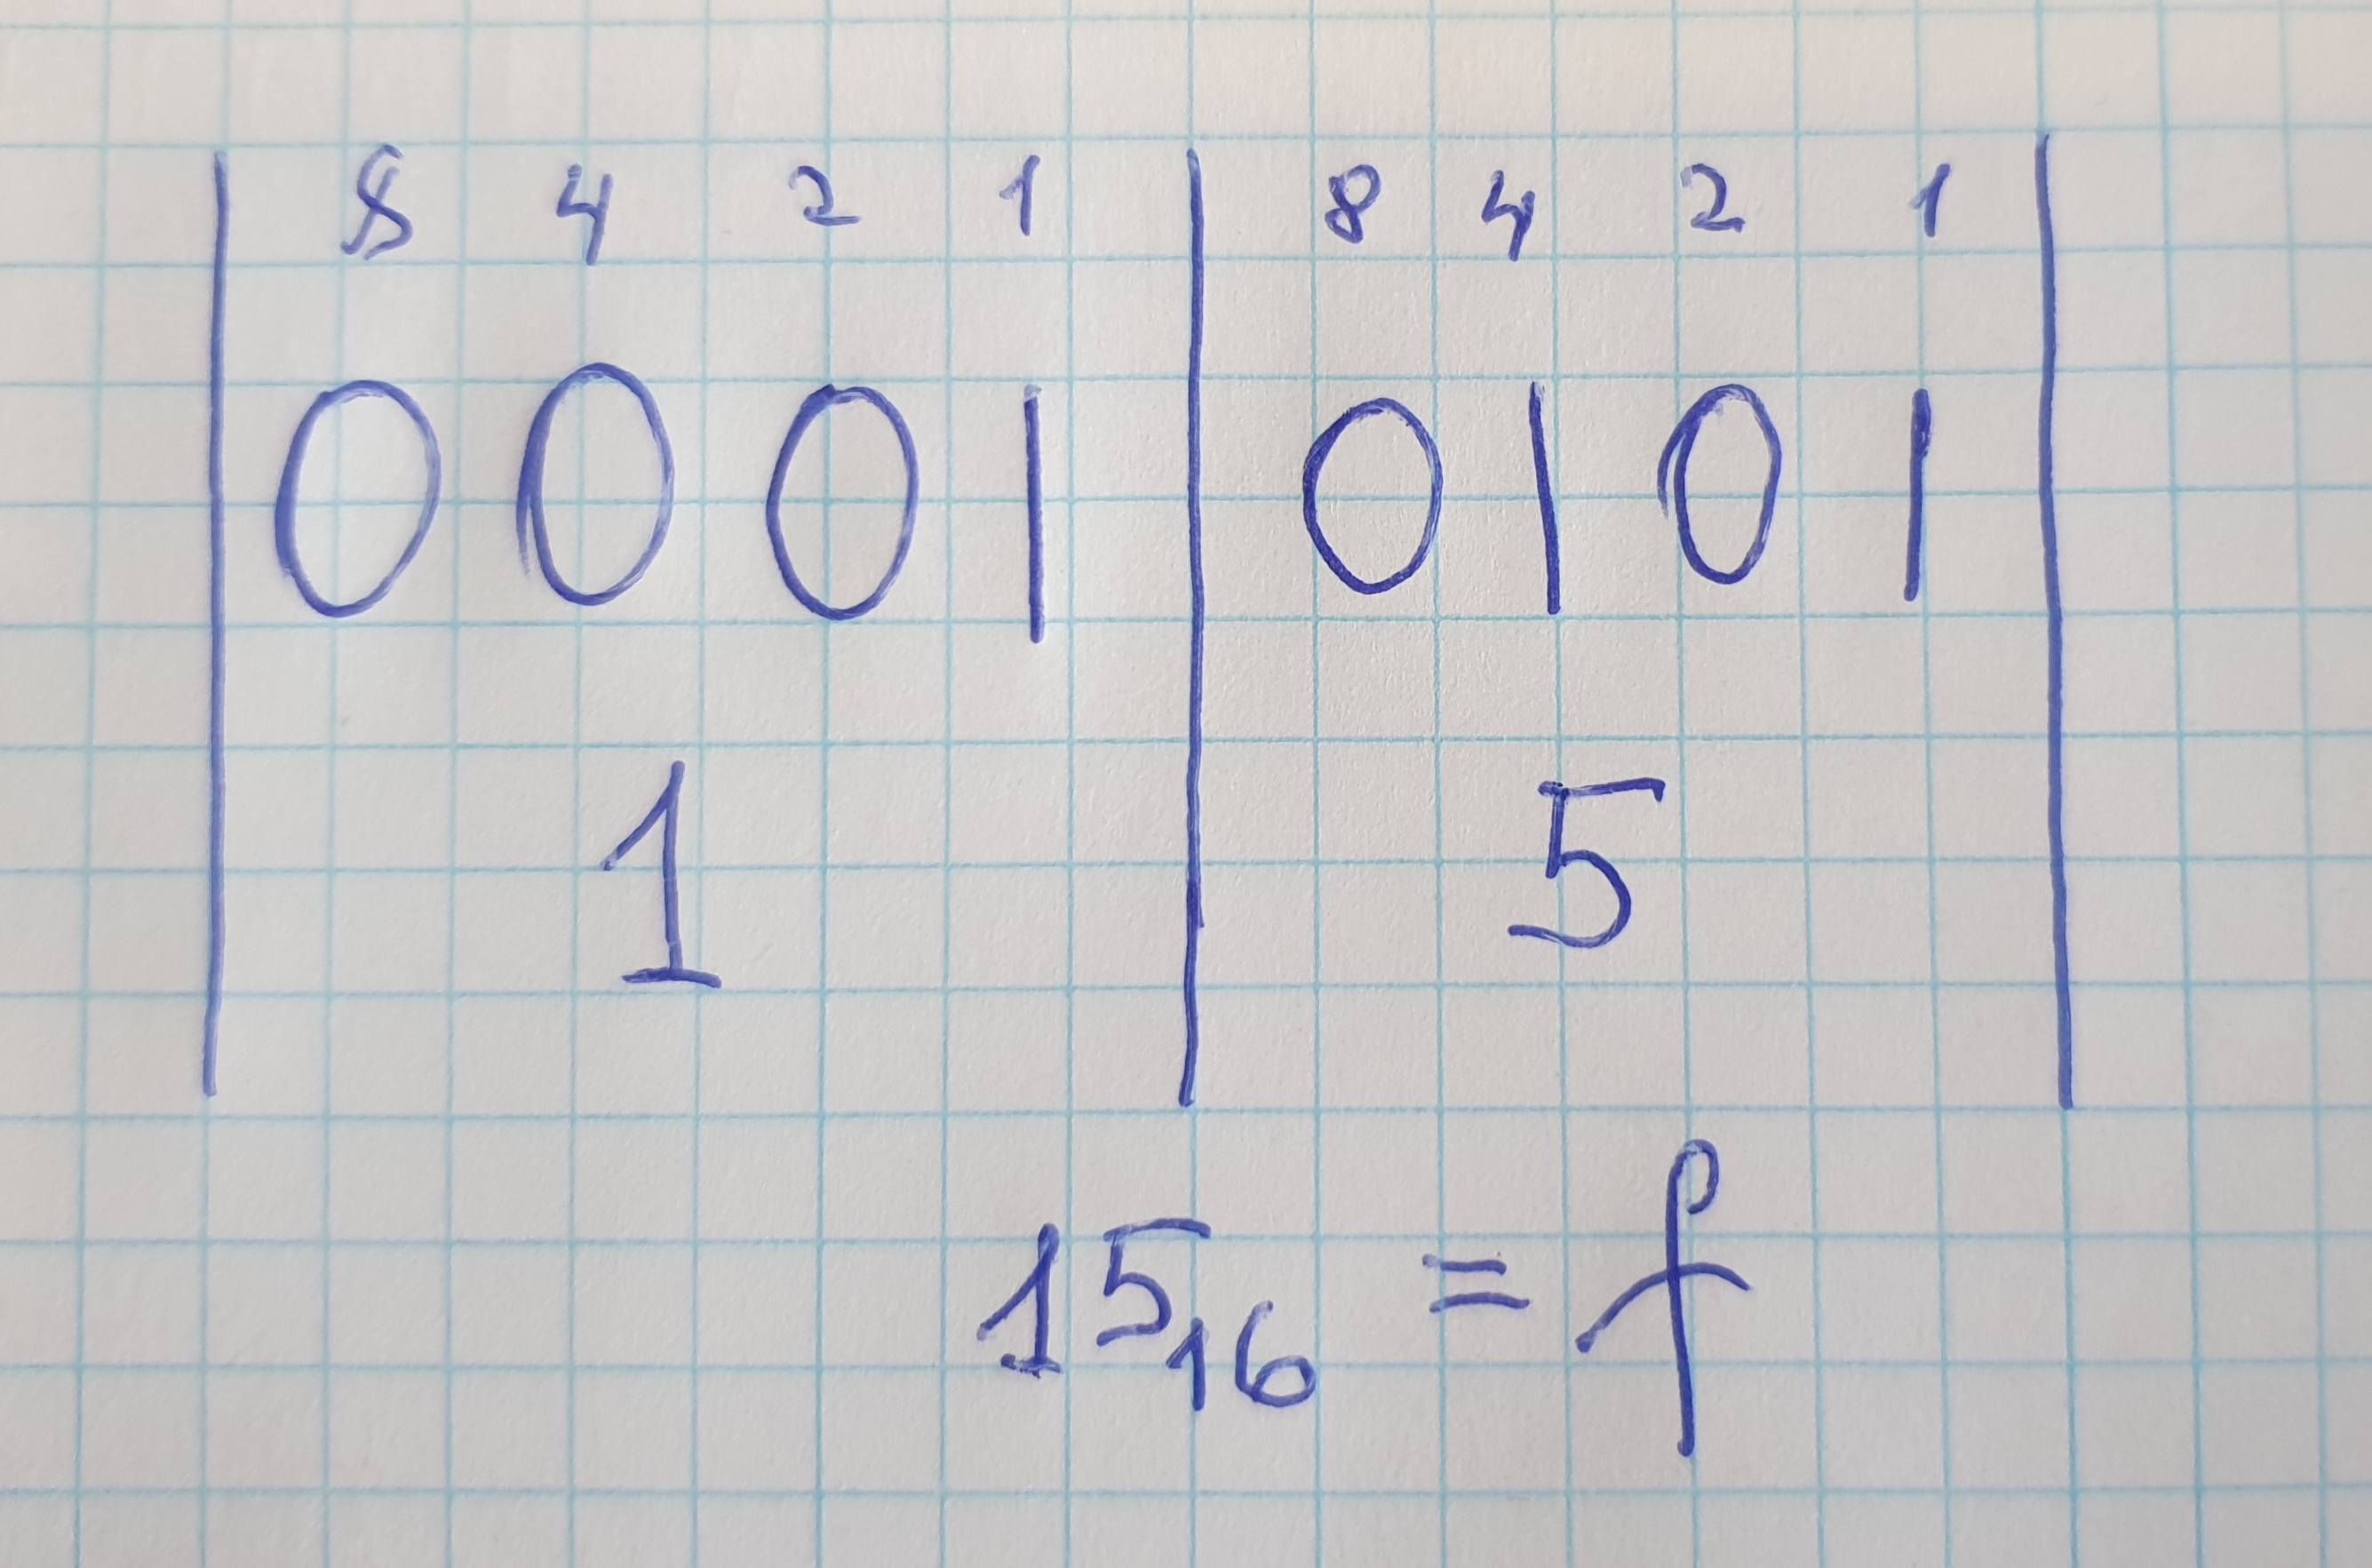
\includegraphics[scale=0.1]{Binary_to_hexadecimal.jpg}
 \caption{Binary to hexadecimal}
 \label{output5}
\end{figure}
\newline
Consider Figure \ref{output6} for a pen-and-paper calculation of the conversion procedure from a hexadecima to binary.
\begin{figure}[h!]
  \centering
 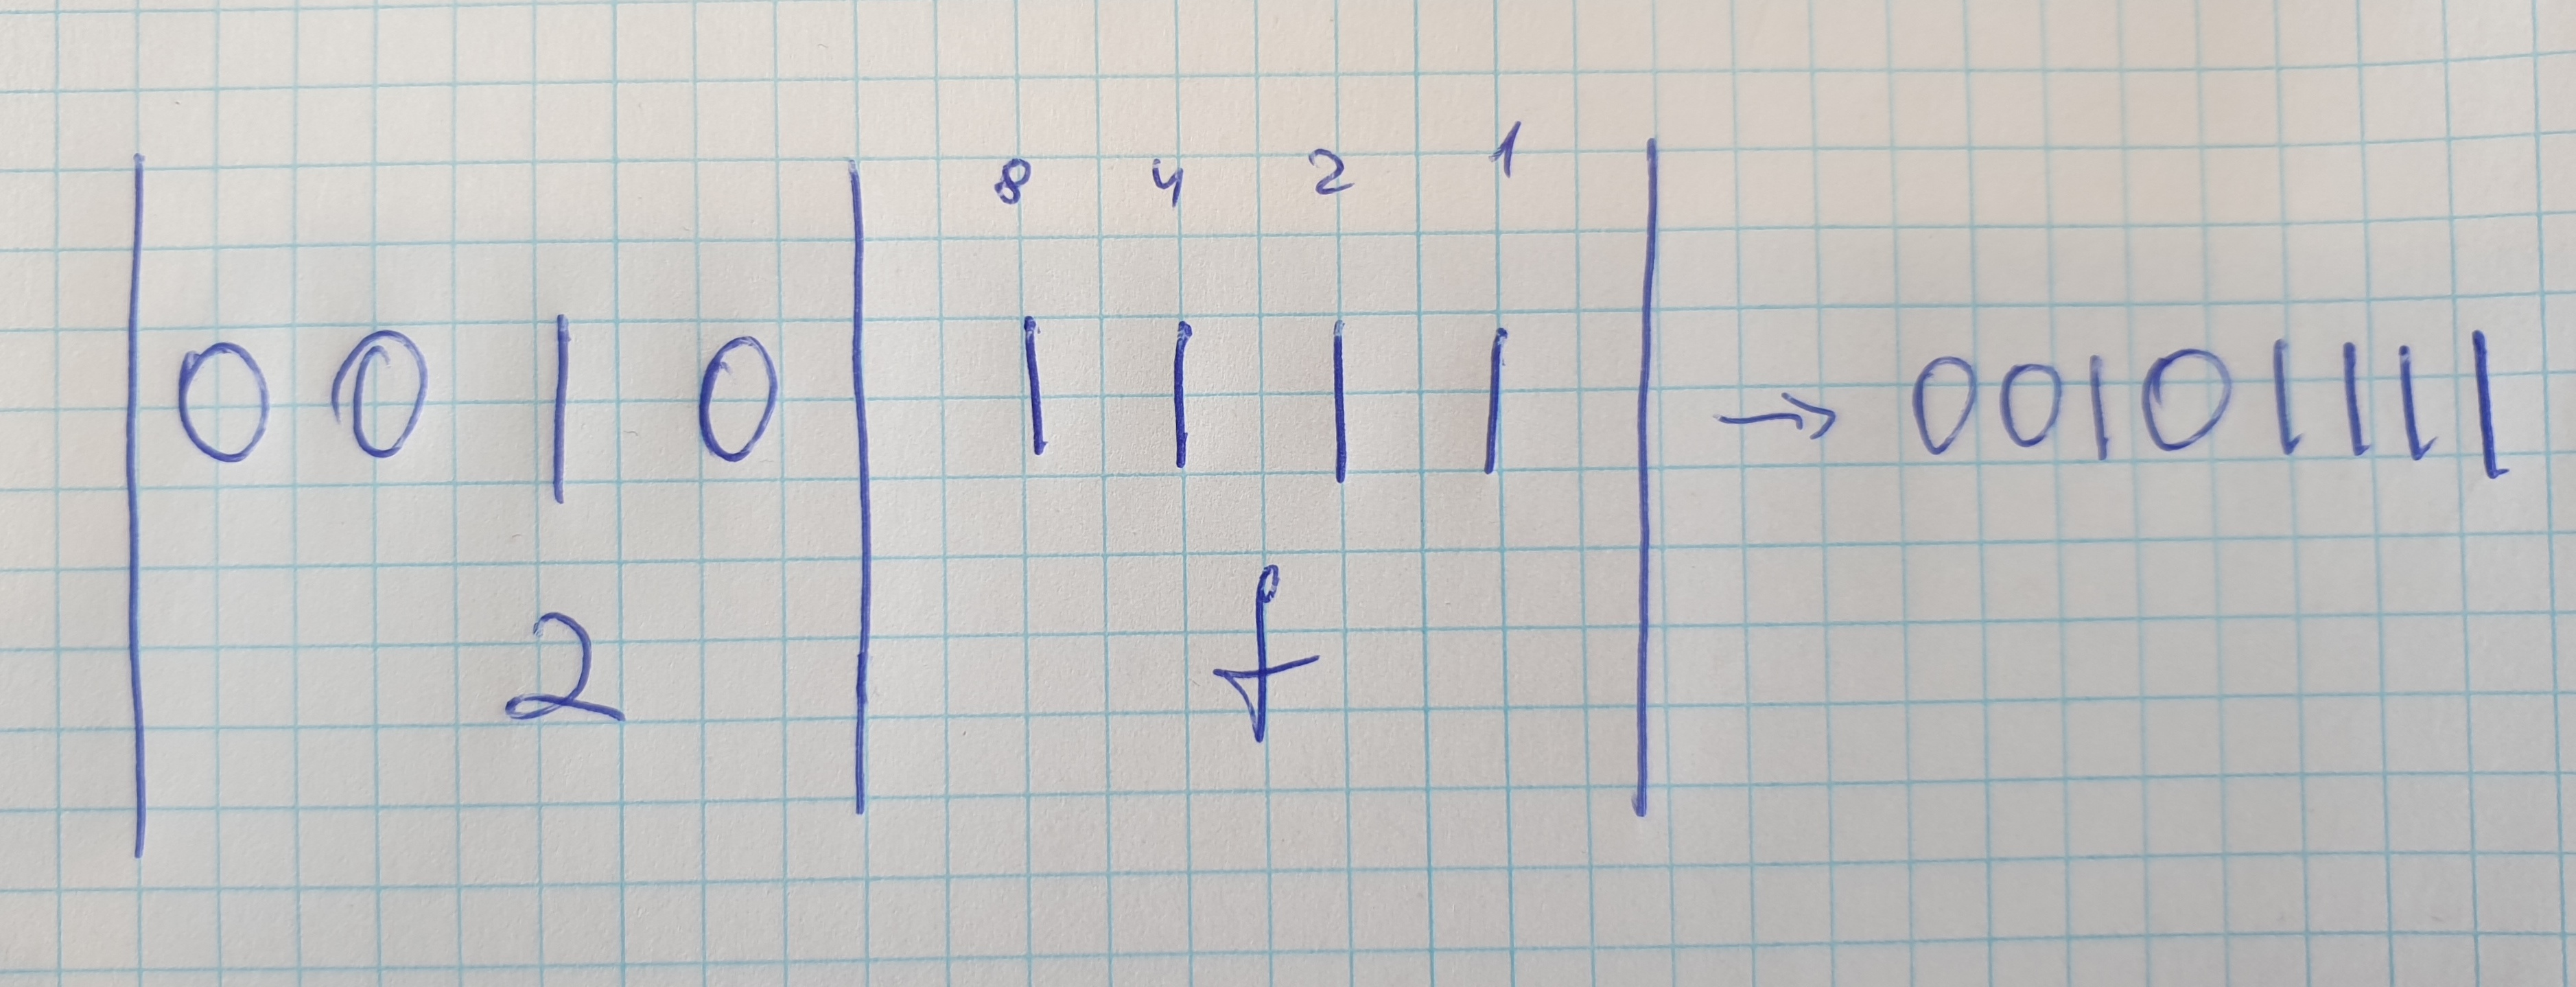
\includegraphics[scale=0.1]{Hexadecimal_to_binary.jpg}
 \caption{Hexadecimal to binary}
 \label{output6}
\end{figure}
\newline
Consider Figure \ref{output7} for a pen-and-paper calculation of the conversion procedure from a binary to octal.
\begin{figure}[h!]
  \centering
 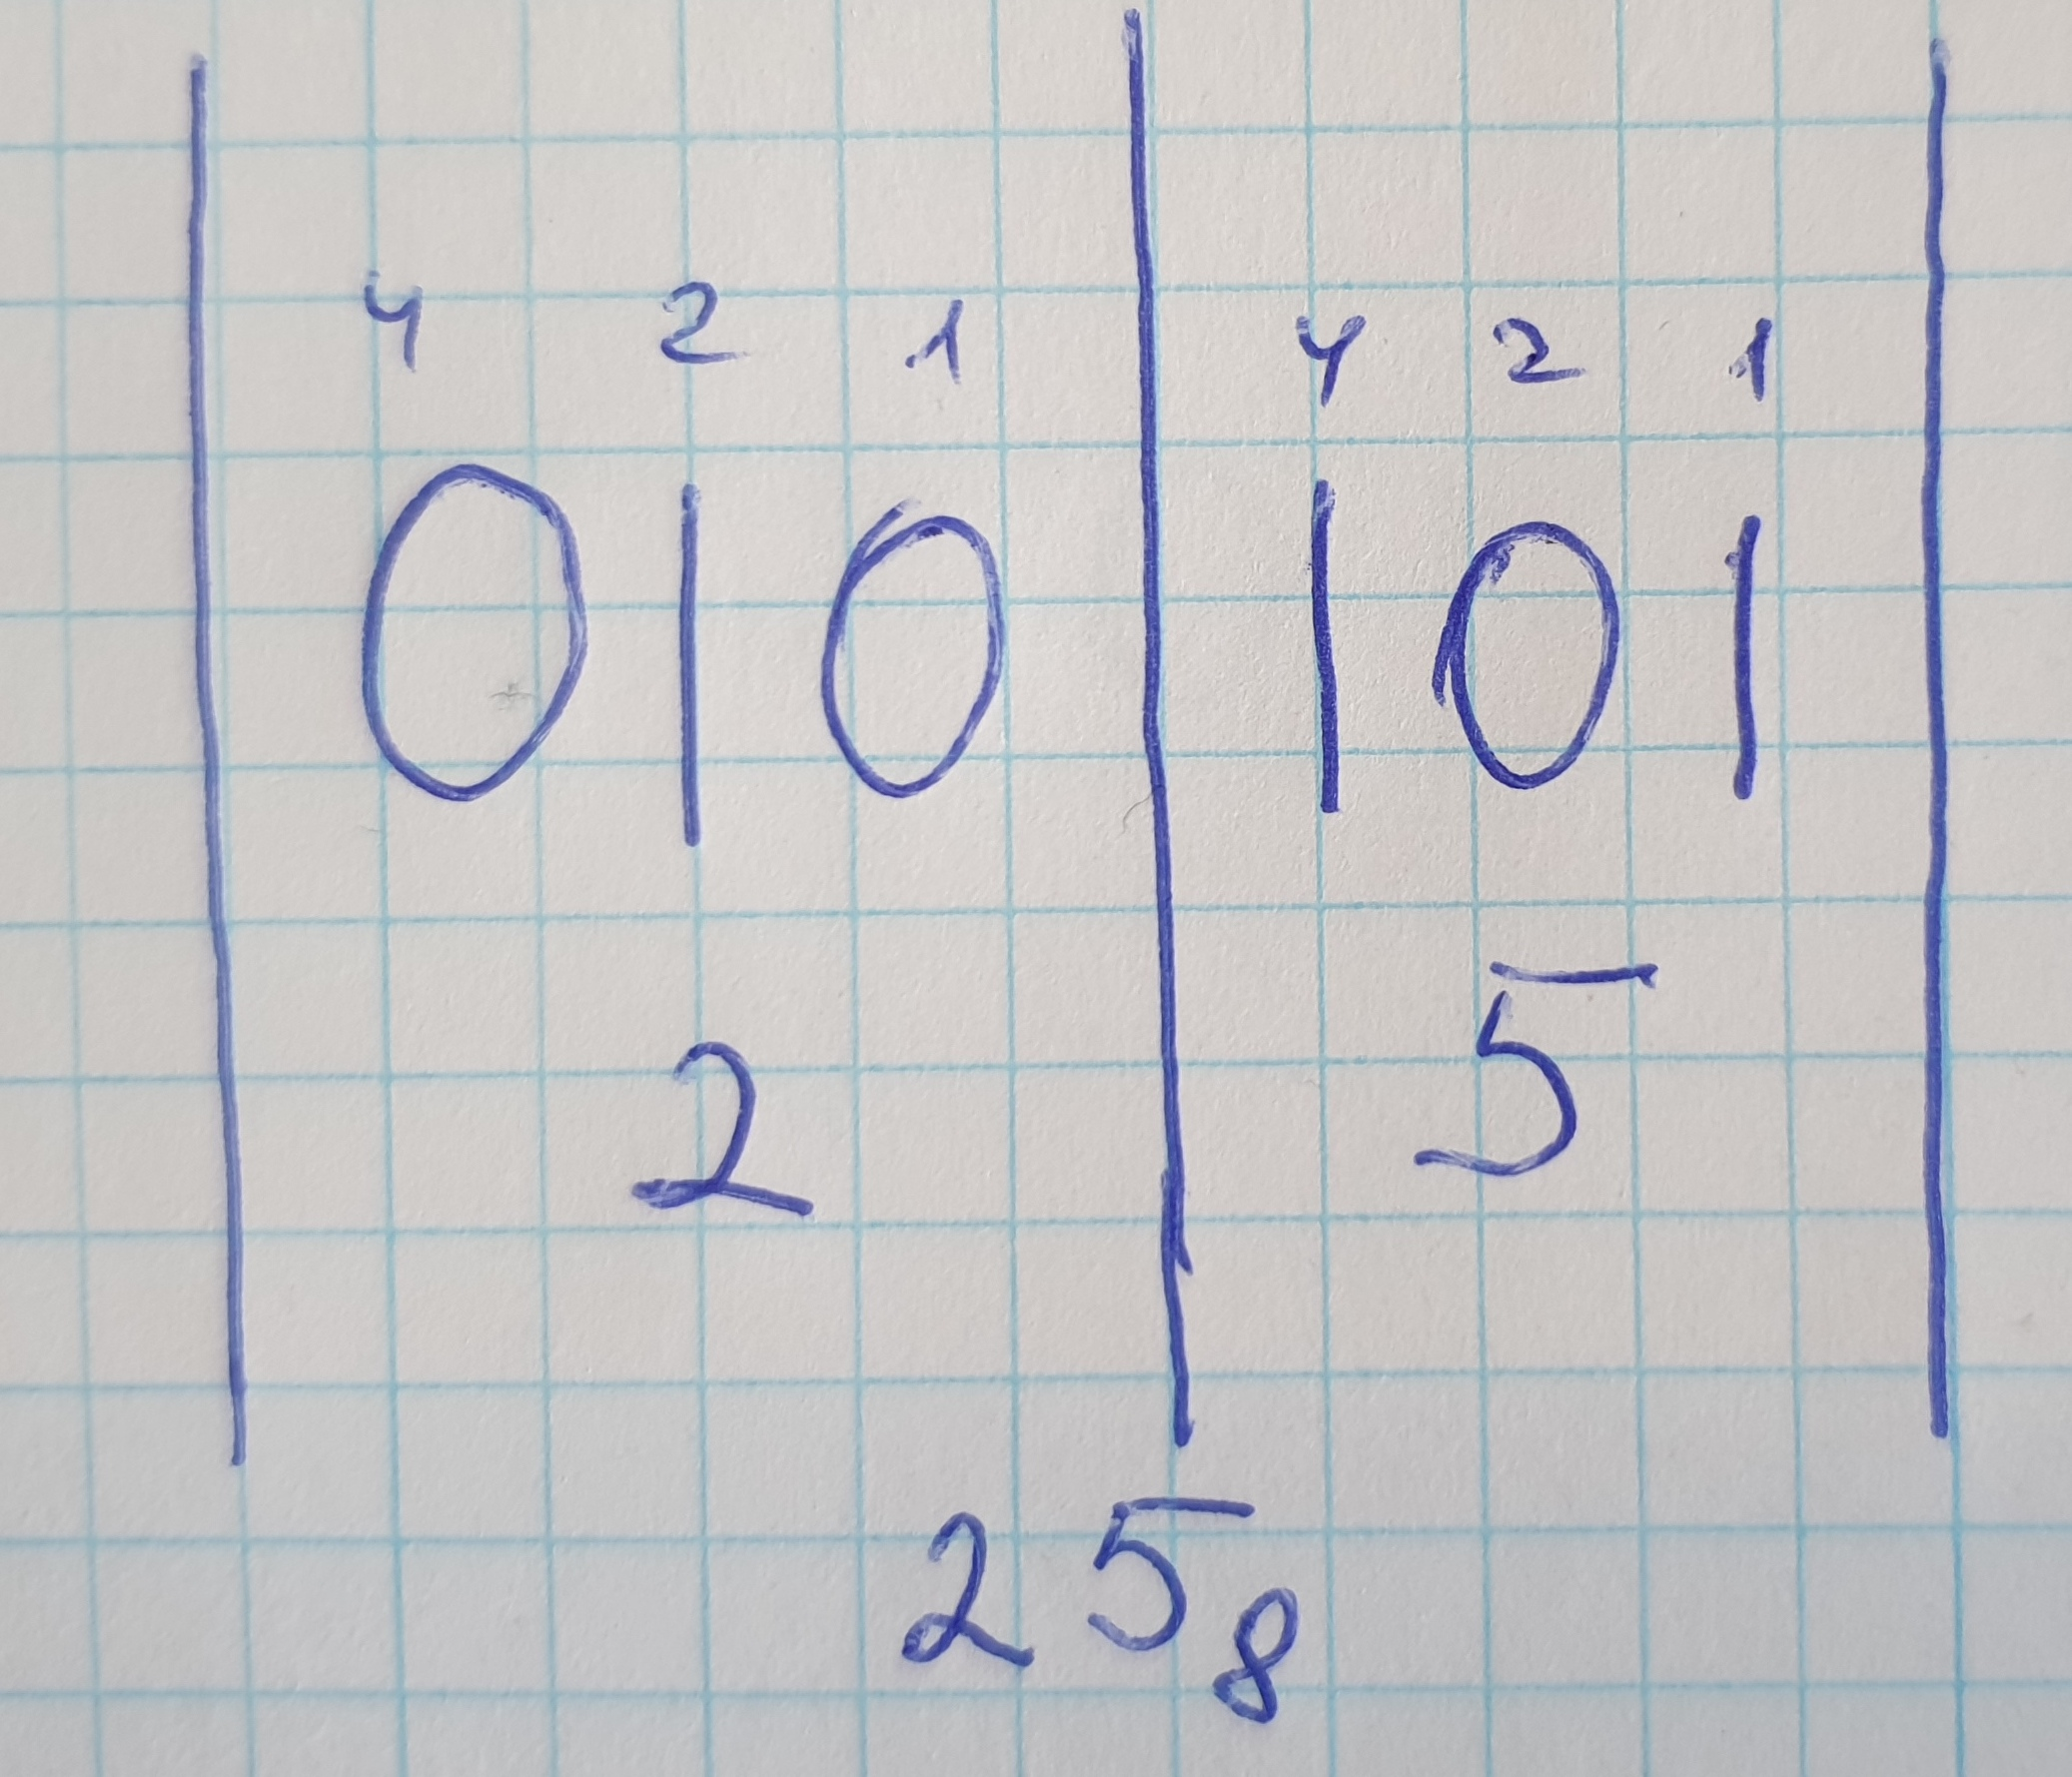
\includegraphics[scale=0.1]{Binary_to_octal.jpg}
 \caption{Binary to octal}
 \label{output7}
\end{figure}
\newline
Consider Figure \ref{output8} for a pen-and-paper calculation of the conversion procedure from an octal number to binary.
\begin{figure}[h!]
  \centering
 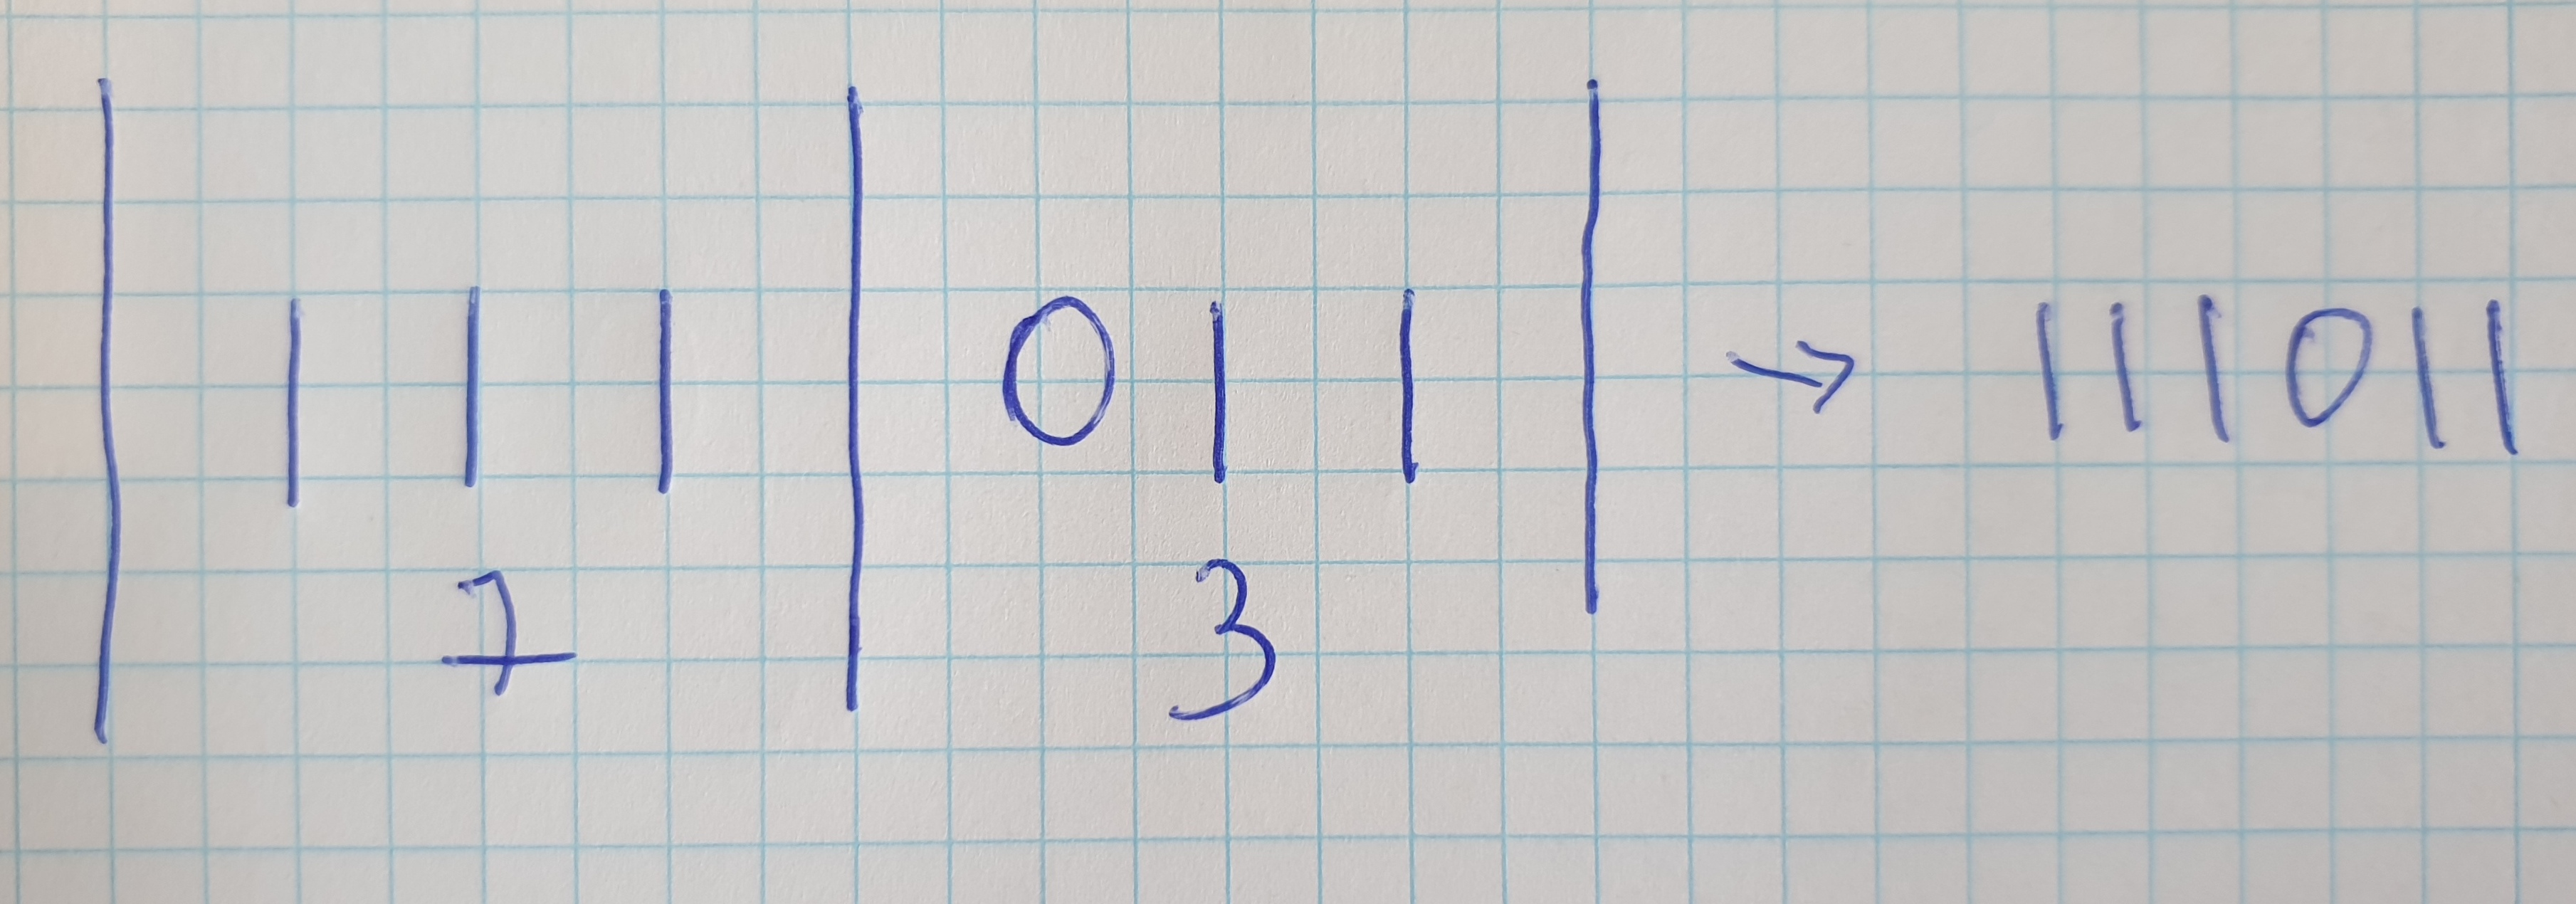
\includegraphics[scale=0.1]{Octal_to_binary.jpg}
 \caption{Octal to binary}
 \label{output8}
\end{figure}

\section{References}
\begin{enumerate}
\item The divide-by-two algorithm in Jon Sporring, \emph{Learning to program with F\#}, Chapter 5, 2019, p. 47.
\item Instruction videos on Youtube: \href{https://www.youtube.com/watch?v=D_YC6DSPpQE}{Link to a YouTube-video}
  \end{enumerate}
  
\end{document}
